\documentclass{article} % For LaTeX2e
\usepackage{nips14submit_e,times}
\usepackage{hyperref}
\usepackage{cite}
\usepackage{url}
\usepackage{graphicx}
\usepackage{float}
\usepackage{amsmath}
\usepackage{amssymb}
\usepackage{pgfplots}
\usepackage{verbatim}

\title{Final Paper : \\Freesound General-Purpose Audio Tagging Challenge}


\author{
Sarah Gross \\
Master of Advanced Computing \thanks{\url{http://ac.cs.tsinghua.edu.cn/}}\\
Tsinghua University\\
\texttt{leihy17@mails.tsinghua.edu.cn} \\
\And
Usama Zafar\\
Master of Advanced Computing\\
Tsinghua University\\
\texttt{zafaru10@mails.tsinghua.edu.cn} \\
}


\newcommand{\fix}{\marginpar{FIX}}
\newcommand{\new}{\marginpar{NEW}}

%\nipsfinalcopy % Uncomment for camera-ready version

\begin{document}


\maketitle

\begin{abstract}
	Sound tagging has been studied for at least a couple of decades now. Among the different types of sounds the most prevalent research areas have been music, speech and enviromental sounds. Some sounds are distinct and instantly recognizable, like a baby's laugh or the strum of a guitar. Other sounds aren't clear and are difficult to pinpoint, or are drowned in a mix of sounds that are difficult to identify individually.\\
	\newline
    Partly because of the vastness of sounds we experience, no reliable automatic general-purpose audio tagging systems exist. Currently, a lot of manual effort is required for tasks like annotating sound collections and providing captions for non-speech events in audiovisual content.\\
	\newline
    This project's goal is to be able to recognize an increased number of sound events of very diverse nature, and to leverage subsets of training data featuring annotations of varying reliability.
\end{abstract}

\section{Introduction}
    Our life is surrounded by various sounds: speech, music, animal call, aircraft, traffic, even the sound of typing words, clicking the mouse, etc. Sounds can be roughly grouped into three clusters: human voice, artificial sound, and non-artificial/natural sound.\\
    \newline
    Human voice refers to sounds created by people physically such as speech, cough, and singing. Artificial sounds refer to sounds created by human activities such as traffic, aircraft, and music. Non- artificial sounds include sounds created by nature such as wind, rain, land animal, insects and marine life.\\
    \newline
    Sound event classification has traditionally benefitted from advances in more mature research in related areas, such as automatic speech recognition (ASR). Detecting sound events in noise is potentially very useful in daily life, such as in allowing a computer to hear and eventually understanding environmental sounds like a human, and from this to infer what is happening in the environment. This technology has implications for improving ASR in many noisy real world scenarios, in security and healthcare monitoring, in intelligent building or city management, and in environmental analysis.
    \newline
    Initially, people classified and documented all information manually. With the development of machine technology, especially the computer science, people started to study new ways of automatic tagging, not only due to its accuracy but also due to its performance. A lot of classification work has been solved efficiently for music, speech and environmental sounds.\\
    \newline
    However, despite the good performance, these automatic tagging machines still need information from the metadata of targets, and present several flaws. This is why there is a need for more reliable general purpose tagging systems.\\

    The aim of this paper is to propose an efficient classification system of environmental sounds, based on Neural Networks. After presenting a literature review of the performances in this field, we will detail our method for feature extraction and sound classification, and expose the results obtained with our method.
    
\section{Related works}
 	Earlier work in the domain of audio signal processing has focused on three broad categories music, speech and environmental sound tagging individually, there has almost been very little to no work in the direction of a unified general purpose sound tagger that would work across these spectrums.
    The main difficulty, is our case, is dealing with sounds with very large bandwith, no structure --- in opposite to human speech ---, bearing possible noise. These differences make the usual sound classification techniques, such as Hidden Markov Models (HMM) or Gaussian Mixture Models (GMM), be much less accurate with this kind of data.


    While Cowling et. al. \cite{Cowling} and Zhang et. al. \cite{Zhang} reject alltogether the idea of using HMM and concentrale on less conventional classification algorithms, Dufaux et. al. \cite{Dufaux} present good results robust to the presence of noise with both HMM and GMM, with around 98\% success with little noise and 57\% in average for maximum noise. However, they needed to aggregate models for each noise level in order to acheive an algorithm working in any noise environement, making the computation time much longer. On the other hand, Casey \cite{Casey} focused on using decorrelated spectral features coupled with HMM for computing similarity and generating source classifications. His work has been incorporated into the MPEG-7 international standard. 

    As for GMM, Cowling et. al. \cite{Cowling} show the huge gap between the performance for music instruments and general non-speech noice, with 90\% for the first, but at most 46\% for the latter.
    
    Duan et. al. \cite{Duan} and Chachada et. al. \cite{Chachada} performed a survey of enviromental sound recognition techniques. Chu et. al. \cite{Chu1} made a selection of appropriate features for environmental sound recognition and furthermore presented \cite{Chu2} a system for environmental sound tagging with time-frequency audio features.

    Though these results are encouraging, they fail to classify with more than 60\% accuracy sounds belonging to many categories with a lot of noise.
    Since environmental sound is unstructured and has a kind of random composition, some authors propose to take inspiration from other well-known unstructured data --- images --- to build efficient classification. 
    Toyoda et. al. \cite{Toyoda} show that Neural Networks give similar results on general sound classification than HMM for less computation.
    Most recently, many papers focused on the use of Convolutional Neural Nets (CNN). Piczak et. al. \cite{Piczak} test their CNN on 3 datasets using different result aggregation procedures (probability, majority vote, ...), and gets an average score of 0.69 across all datasets.\\
    With CNN, Zhang et. al. \cite{Zhang} get highly reliable results from NOISEX-92 database with 92,15\% mean accuracy, its strong point being correct despite the noise in the audio samples.

\section{Method}

	\subsection{Feature extraction}
		In sound analysis, the raw samples are very complex and it is difficult to get valuable information directly from them, especially if they contain noise.
		Feature extraction is a process to extract a subset of features to be used for training. Feature extraction can be carried out for any number of reasons some of which are (but not limited to), to reduce the amount of resources required to describe large set of data, remove redundancy, get best set of features, etc.

		\textbf{Mel Frequency Cepstral Coefficents (MFCCs)} are a feature widely used in automatic speech and speaker recognition. They were introduced by Davis and Mermelstein in the 1980's, and have been state-of-the-art ever since. Prior to the introduction of MFCCs, Linear Prediction Coefficients (LPCs) and Linear Prediction Cepstral Coefficients (LPCCs) and were the main feature type for automatic speech recognition (ASR), especially with HMM classifiers.\\

		\begin{figure}[H]
		\centering
		  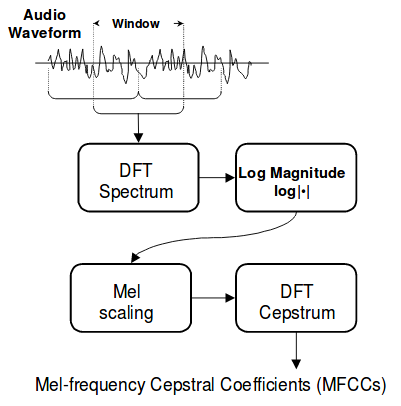
\includegraphics[width=0.5\linewidth]{steps_mfcc.png}
		  \caption{Flowchart for MFCC extraction}
		  \label{fig:mfccflowchart}
		\end{figure}

		Typical steps involved with extracting mfcc features of an audio signal \ref{fig:mfccflowchart} are as follows:
		\begin{enumerate}
		    \item \textbf{Frame the signal into short frames}.  An audio signal is constantly changing, so to simplify things we assume that on short time scales the audio signal doesn't change much (when we say it doesn't change, we mean statistically i.e. statistically stationary, obviously the samples are constantly changing on even short time scales). 
        We call our time domain signal $s(n)$. Once it is framed we have $s_i(n)$ where n ranges over 1 to $N$ samples and $i$ ranges over the number of frames. When we calculate the complex DFT, we get $S_i(k)$ - where the $i$ denotes the frame number corresponding to the time-domain frame. $P_i(k)$ is then the power spectrum of frame $i$.\\
		    \item \textbf{For each frame calculate the periodogram estimates of the power spectrum}. This modelizes the way human ear transmits information to the brain.\\\\
		We first make a Discret Fourier Transform of the frame:\\
		$$S_i(k) = \displaystyle\sum_{n=1}^N s_i(n)h(n)e^{j2\pi kn /N}, \quad 1 \leq k \leq K$$
		where $h(n)$ is an $N$ sample long analysis window (e.g. hamming window), and $K$ is the length of the DFT.\\
		Then we get periodogram-based power spectral estimate for the speech frame $S_i(n)$ by taking the absolute value of the complex fourier transform and square the result:\\
		$$P_i(k) = \frac{1}{N} |S_i(k)|^2$$
		    \item \textbf{Apply the mel filterbank to the power spectra, sum the energy in each filter}. The Mel-spaced filterbank  is a set of 20-40 (26 is standard) triangular filters that we apply to the periodogram power spectral estimate from step 2. Each vector is mostly zeros, but is non-zero for a certain section of the spectrum. \\\\
		For instance, the first filterbank will start at the first point, reach its peak at the second point, then return to zero at the 3rd point. The second filterbank will start at the 2nd point, reach its max at the 3rd, then be zero at the 4th etc.
		We convert frequency from Hz to Mel using the formula :
		$$ M(f) = 1125 ln(1 + f/700) $$
		Then, to calculate filterbank energies we multiply each filterbank with the power spectrum, then add up the coefficents.

		    \item \textbf{Take the logarithm of all filterbank energies.}
		    \item \textbf{Take the DCT of the log filterbank energies.}
		    \item \textbf{Keep DCT coefficients 2-13, discard the rest.}
		\end{enumerate}

		We perform feature extraction with the python library \verb+LibROSA+ \ref{fig:mfccgraph}. Along with MFCC, we extract other userful features \textit{chroma, mel, contrast, tonnetz} to make better distinction between the audio files.\\
		Since we had huge amount of data approximately 18000+ audio files, the process of feature extraction took 5-6 hours to complete. In order to handle this issue we implemented multi-threaded environment to extract features. We assign each thread a workload of 500 files and fire them all up in parallel. Through this approach we were successful in bringing down the extraction time from 6 hours to 1 hour approximately.\\
		In addition to multi-threading, we store features in files in order to be able to run classification several times witout needing to compute again feature extraction.

		\begin{figure}[H]
		  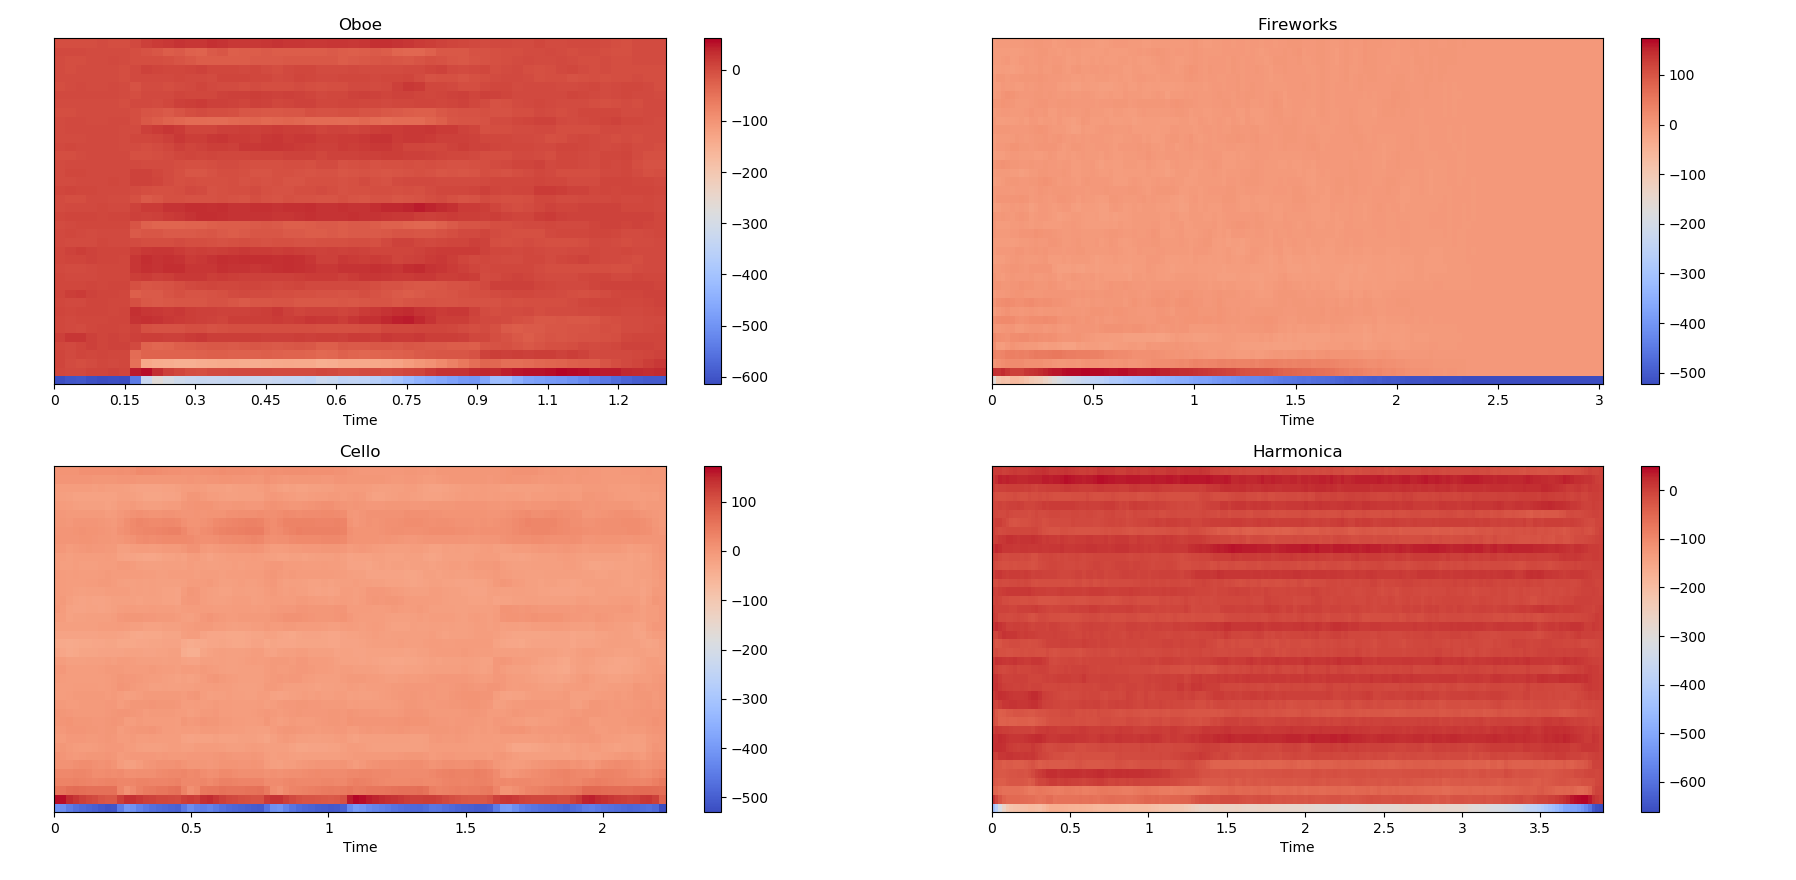
\includegraphics[width=\linewidth]{mfcc.png}
		  \caption{Mel Frequency Cepstral Coefficients plot for a few audio samples}
		  \label{fig:mfccgraph}
		\end{figure}
        

	\subsection{Sound classification}

		After extracting the features, they are fed to a neural network.
		We used \verb+Tensorflow+ to implement a multilayer neural network. We used the following settings :

		\vskip2ex
		\begin{table}
		\centering
		\caption{Tensorflow MNN settings}
		\begin{tabular}{ccccc}
		\hline\hline
		Parameter & Chosen value\\
		\hline
		Number layers & 3\\
		Neurons per layer & \{200, 250, 300\}\\
		Act func per layer & \{tanh, sig, sig\}\\
		Learning rate & 0.005 (exp decay)\\
		Cost function & cross entropy\\
		Optimize & adam\\ 
		Num epochs & 500\\
		\hline\hline
		\end{tabular}
		\end{table}
		\vskip2ex

		These settings were obtained by try-and-fail run of code :
		\begin{itemize}
			\item Toyoda et. al \cite{Toyoda} use 3 layers with \{48, 32, 2\} neurons. This gave a fast-converging network, however the cost was very high. On the opposite, putting \{280, 200, 300\} neurons prevented the MNN from converging with data larger than 1000 items. This is why we decreased to the final values in Table 1.
			\item We originally took a learning rate of 0.01 based on our experience of neural nets. However the mnn would not converge this way for large dataset, this is why we gradually decreased it and used exponential decay.
			\item We first used gradient descent optimized, but got better results with adam.
			\item 500 or 1000 number of epochs give similar results.
		\end{itemize}

		After MNN, we implemented a 2D Convolutional Neural Network in order to compare and combine the techniques.\\
		We used Piczak et al. 's settings \cite{Piczak} for windowing by dividing each sound clip into segments of 60x41 (60 rows and 41 columns) \ref{fig:cnngraph}. The mel-spec and their deltas become two channels, which are fed into CNN.\\
		We preferred Python package \verb+Keras+ since CNN implementation with \verb+Tensorflow+, especially concerning windowing step, is cumbersome.

		\vskip1ex
		\begin{figure}
		\centering
		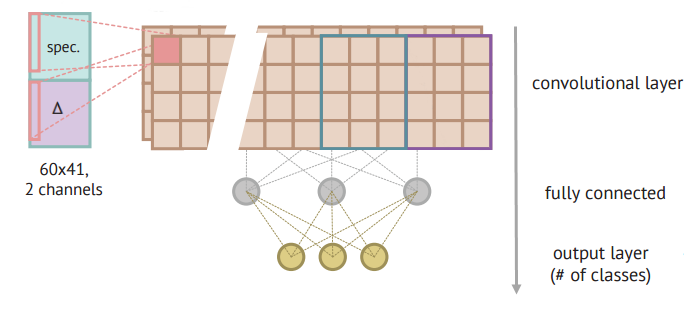
\includegraphics[width=0.9\columnwidth]{cnn_chart.png}
		\caption{Schema of implemented CNN}
		\label{fig:cnngraph}
		\end{figure}
		\vskip2ex

		The 2D CNN is built using the following steps :
		\begin{enumerate} 
			\item The 2D input is reshaped to one dimension.
			\item We have a first convolutional layer. A Convolution layer tries to extract higher-level features by replacing data for each (one) pixel with a value computed from the pixels covered by the e.g. 4×10 filter centered on that pixel(all the pixels in that region). We slide the filter across the width and height of the input and compute the dot products between the entries of the filter and input at each position. "Same" padding means the output size is the same as the input size. This requires the filter window to shift out of the input map. The portions where the filter window is outside of the input map is the padding.
			\item Add ReLU activation function. This transforms the output like so: $ReLU(x) = max(0,x)$.
			\item  We reduce the spatial size of the output by replacing values of every pool (kernel) by the max of those values using "Max" Pooling.
			\item We perform steps 2, 3, 4 three other times
			\item The output is shaped back using \verb+Dense+ function. 
		\end{enumerate}

		----------- TODO USAMA : WRITE THINGS HERE -------------------
		More details about CNN ...

\section{Experiments and results}
	\subsection{Dataset}
		For experimenting our neural networks, we used Freesound Dataset Kaggle 2018 (or FSDKaggle2018 for short), an audio dataset containing 18,873 .wav annotated files from Google's AudioSet Ontology \cite{audioset}.\\
		They can have 41 different labels of various sounds, from instruments to human-origin noise :\\
		\textit{"Acoustic\_guitar", "Applause", "Bark", "Bass\_drum", "Burping\_or\_eructation", "Bus", "Cello", "Chime", "Clarinet", "Computer\_keyboard", "Cough", "Cowbell", "Double\_bass", "Drawer\_open\_or\_close", "Electric\_piano", "Fart", "Finger\_snapping", "Fireworks", "Flute", "Glockenspiel", "Gong", "Gunshot\_or\_gunfire", "Harmonica", "Hi-hat", "Keys\_jangling", "Knock", "Laughter", "Meow", "Microwave\_oven", "Oboe", "Saxophone", "Scissors", "Shatter", "Snare\_drum", "Squeak", "Tambourine", "Tearing", "Telephone", "Trumpet", "Violin\_or\_fiddle", "Writing"}.\\

		Some of the files were manually verified. The distribution of manual verification and labels is unequal across the dataset \ref{fig:category_distribution}:
		\begin{figure}[H]
		  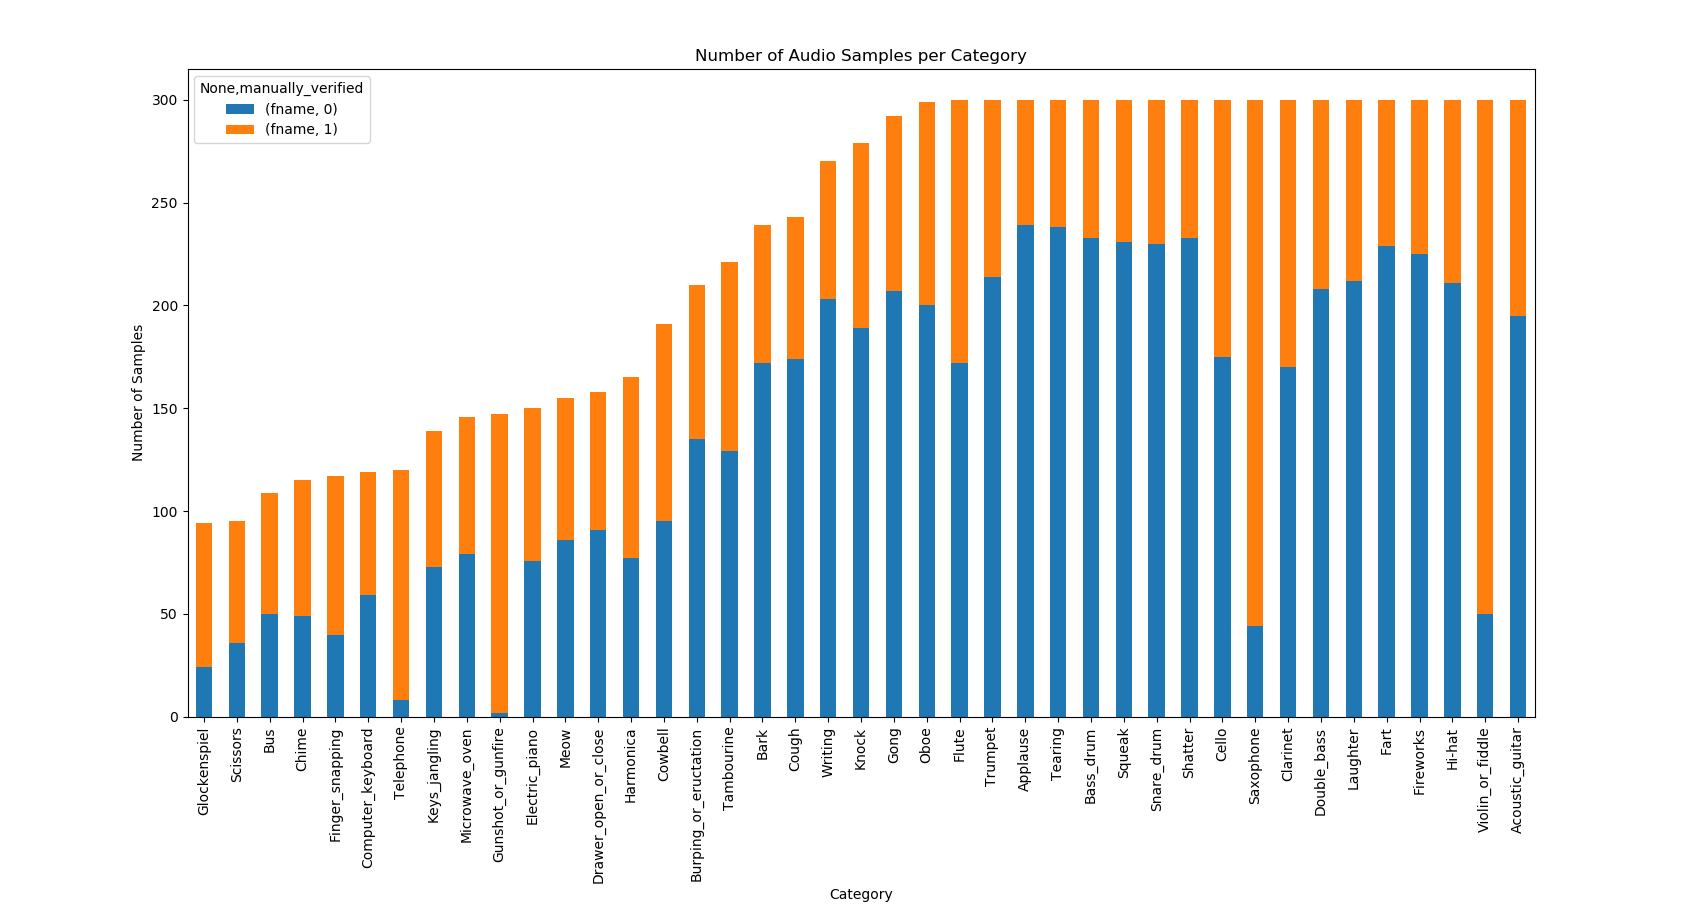
\includegraphics[width=\linewidth]{../midterm/category_distribution.png}
		  \caption{Distribution of samples per category}
		  \label{fig:category_distribution}
		\end{figure}


	\subsection{Evaluation}
		For each sound file, we give maximum 3 most likely labels.
		Submissions are evaluated according to the Mean Average Precision @ 3 (MAP@3):

		$$MAP@3 = \frac{1}{U} \displaystyle\sum_{u=1}^U \displaystyle\sum_{k=1}^{min(n,3)}P(k)$$\\

		where $U$ is the number of scored audio files in the test data, $P(k)$ is the precision at cutoff k and $n$ is the number of given labels.

	\subsection{Results}

		This graph shows the score output by Kaggle using the metric previously evoked.\\
		Perfecting the settings of the multilayer neural network makes our score constantly improve over the submissions.
		\vskip1ex
		\begin{center}
		\begin{tikzpicture}
		\centering
            \begin{axis}[width=0.90\columnwidth, height=200, ylabel=Score, xlabel=Submission]
                \addplot[thick, teal] table [x=submission, y=score, col sep=comma ] {submissions.csv};
            \end{axis}
        \end{tikzpicture}
        \end{center}
        \vskip2ex

        Our MNN loss smoothly goes down until approximately reaching 0.5. The variation is strictly monotonic, which shows that we keep reaching towards the optimum without going over it.\\
        Compared to other loss functions, using cross-entropy speeds up the decreasing rate of the cost.
        \vskip2ex
		\begin{center}
		\begin{tikzpicture}
		\centering
            \begin{axis}[width=0.90\columnwidth, height=200, ylabel=Cost, xlabel=Num of epochs]
                \addplot[thick, teal] table [x=epoch, y=cost, col sep=comma, ] {cost_history_mnn.csv};
            \end{axis}
        \end{tikzpicture}
        \end{center}
        \vskip2ex

        In order to understand better the performance of our classification algorithm, the confusion matrix \ref{fig:confusion_matrix} is built for the 10 most frequent labels : Acoustic\_guitar, Clarinet, Double\_bass, Fart, Fireworks, Hi-hat, Laughter, Saxophone, Shatter, Violin\_or\_fiddle.\\
		\begin{figure}
		\centering
		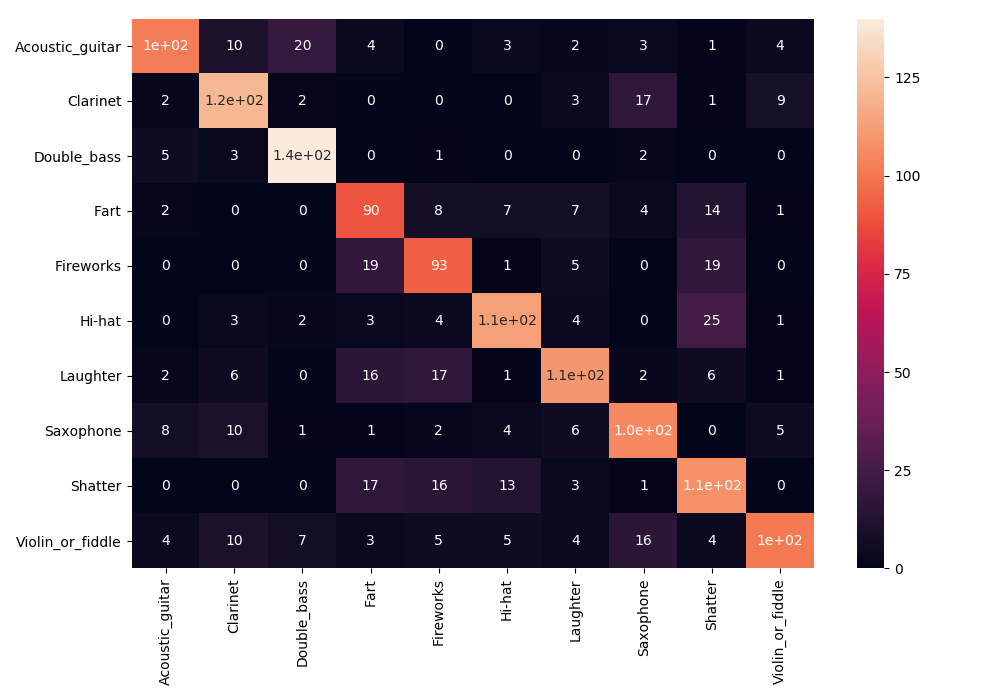
\includegraphics[width=0.99\columnwidth]{confusion_matrix_full.png}
		\caption{Confusion Matrix (x axis : prediction, y axis : true label)}
		\label{fig:confusion_matrix}
		\end{figure}
		\vskip2ex

		We notice that, like in Cowling et al.'s case \cite{Cowling}, the model makes less mistakes on the musical instruments than on the other sounds (Fart, Fireworks, Shatter) which are sometimes confused together. Shatter and Hi-Hat are also often mixed up, which is quite logical due to the similarity of there two sounds.\\
        Still, even though they are all non-musical sounds, Shatter has much better statistics than Fart of Fireworks. Piczak et. al. \cite{Piczak} notice that short-scale temporal samples perform worse than the others, however Fireworks samples are usually about the same length as Shatter, therefore this reason seems unlikely. One hypothesis could be that low-frequency samples (Fart, Fireworks) perform worse than those with high frequency like Shatter.



        ----------- TODO USAMA : WRITE THINGS HERE -------------------
        Some results about CNN ...




\section{Conclusion}

	This work presents a classification method of environmental sounds based on neural networks. A multi-threaded feature extraction process has been developped to get valuable spectral information within an hour. After incremental trials, we build a robust yet simple multilayer neural network running almost instantaneously producing very low cost. Using MAP@3 metric with 3 most likely labels, it classifies correctly 56,4\% of the data, which is a score similar to previous works on HMM \cite{Dufaux} and multilayer neural networks \cite{Toyoda}.\\
	Yet, a better implementation of CNN would have probably improved significantly our results, and might have helped us reach the impressive scores of Zhang et. al. \cite{Zhang}.

\subsubsection*{Acknowledgments}
	We are grateful to Tsinghua University's Department of Computer Science for providing us the ressources necessary for this project,
	and to Prof. Jun Zhu\footnote{\url{http://ml.cs.tsinghua.edu.cn/~jun/index.shtml}} and Jie Tang for their guidance.

\nocite{*}
\bibliographystyle{unsrt}
\bibliography{project_final}

\end{document}
